\newchapter{commissioning}{Setup and Commissioning of the PFF System}

This is the introductory text.

\newsection{fontSetup}{Feedforward Controller (FONT5a Board)}

\subsection{Cabling Setup}
\label{ss:fontCables}

\subsection{Implementation of PFF Algorithm in Firmware}
\label{ss:pffFirmware}

Not using arcsin in phase reconstruction - effect

Gain conversion factor

\subsection{DAQ and Setup Parameters}
\label{ss:fontDAQ}

gain

filter weights

timing delays

saturate rather than overflow output

Interleaved mode


\subsection{ADC Droop Correction}
\label{ss:droopCorr}

The droop in the response of the FONT5 ADCs, as most clearly seen in the output of the diode channel in Figure \ref{f:diodeDroop} (although it also effects the mixer channel), is not an issue for the work the FONT group does at ATF2 where the signals are well approximated by delta functions separated by \(\sim\)100~ns. Although the droop has been seen previously, its significance for the continuous microsecond length pulse at CTF3 had not been considered because of this.

\begin{figure}
  \centering
  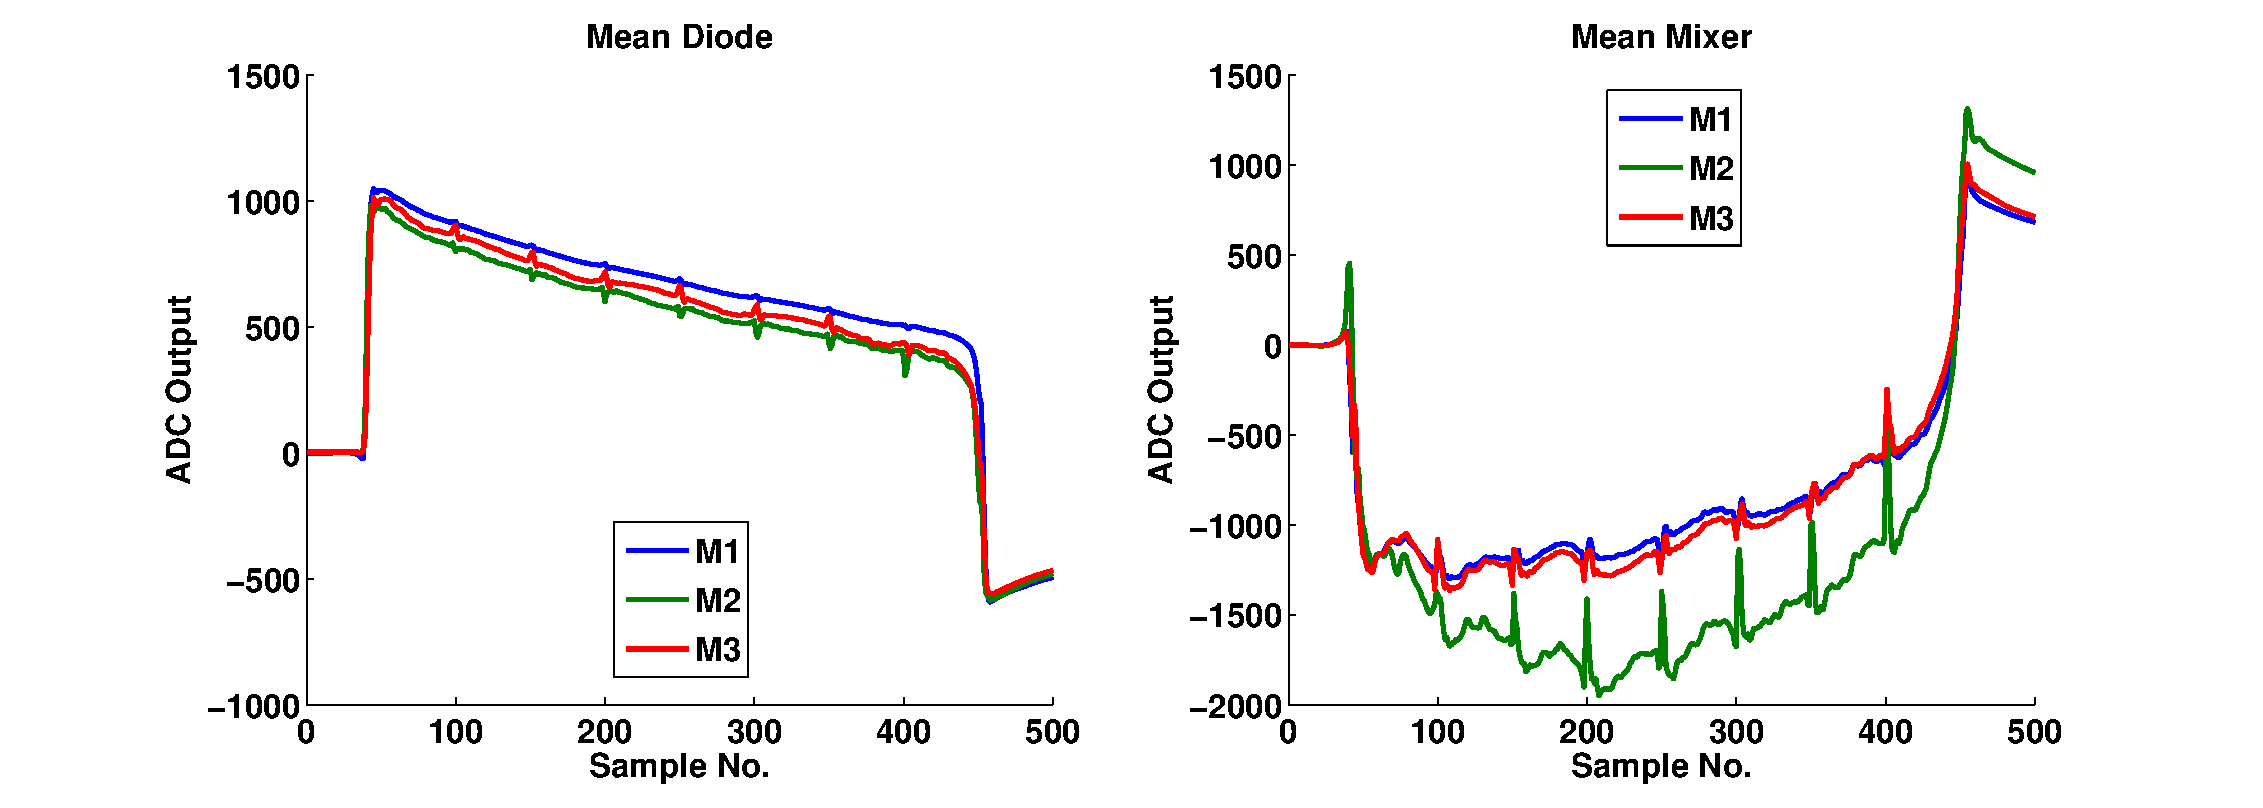
\includegraphics[width=0.9\textwidth]{Figures/commissioning/diodeDroop}
  \caption{Mean diode and mixer output with no filter.}
  \label{f:diodeDroop}
\end{figure}

The droop emerges as a result of the use of AC coupling on the ADC input transformers for electrical isolation. This involves using a capacitor, the current across which is dependent on \({dV}/{dt}\) (\(V\) being voltage and \(t\) time), to remove the DC component from a signal. In particular for the diode channel, which should be a square wave, the output is increasingly well described by a DC signal on the flat top as you move away from the leading edge of the pulse, with the capacitor causing droop in the response as a result.

In the simplest case the droop should be well described by an exponential decay of the form \(A\exp\left(-t/T\right)\). The droop makes it difficult to perform calibrations and measurements on the data and one way in which it could be removed in offline analysis is by determining the decay constants, \(T\), for each of the ADCs on the FONT5 board. To avoid the influence of beam effects tests were done in Oxford using a generated 10~\(\mu\)s DC pulse.

\begin{figure}
  \centering
  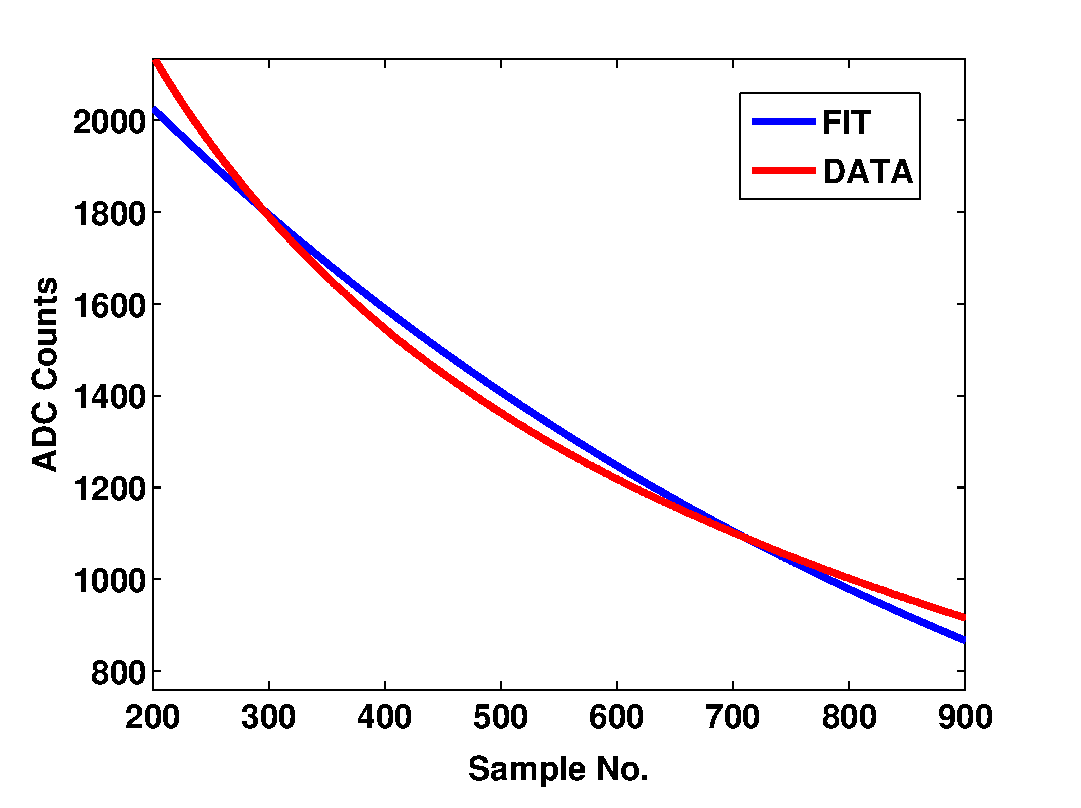
\includegraphics[width=0.45\textwidth]{Figures/commissioning/droopFit}
  \caption{Attempted exponential fit to the ADC droop.}
  \label{f:droopFit}
\end{figure}

Unfortunately, as can be seen in Figure \ref{f:droopFit} which shows an example of an exponential fit for one ADC, although the fits return good \(R^{2}\) values it is clear that the slope of the exponential curve is not a good match for the slope of the data. This is perhaps not unexpected as the ferrite cores used in the transformers have many non-linear properties. In fact, by using a fit with two exponential terms it is possible to obtain a perfect match to the data but at this point the complexity of the fit would make any attempt to remove the droop in real beam data in this way spurious.

Instead, changes will be made to the currently in development FONT5a board hardware and firmware to greatly reduce the scale of the droop. Different transformers will be used to reduce the droop rate by up to a factor of fifty and in addition digital filtering will be implemented in firmware to smooth out and reduce the remaining droop component even further. It is expected that after these changes the droop will be small enough to not have a detrimental effect on the performance of the phase feedforward system. 


\newsection{amplifierSetup}{Amplifier}

\subsection{Introduction}
\label{ss:ampIntro}

Amplifier versions:

First version (nov 2014) 350 V (check)

2nd version  (jul 2015) 650 V - double FETs

3rd version: 1200 V with combiner module (?) not pursued

\subsection{Installation}
\label{ss:ampInstallation}


Amplifier inputs:

Trigger from FONT5a board

DAC1 and DAC2 from FONT5a board


Amplifier outputs:

4 drive signals - one for each strip. Sent to downstream end of kicker (why?)

4 terminators

Amplifier on time monitoring

Monitoring of each amplifier output

\begin{figure}
  \centering
  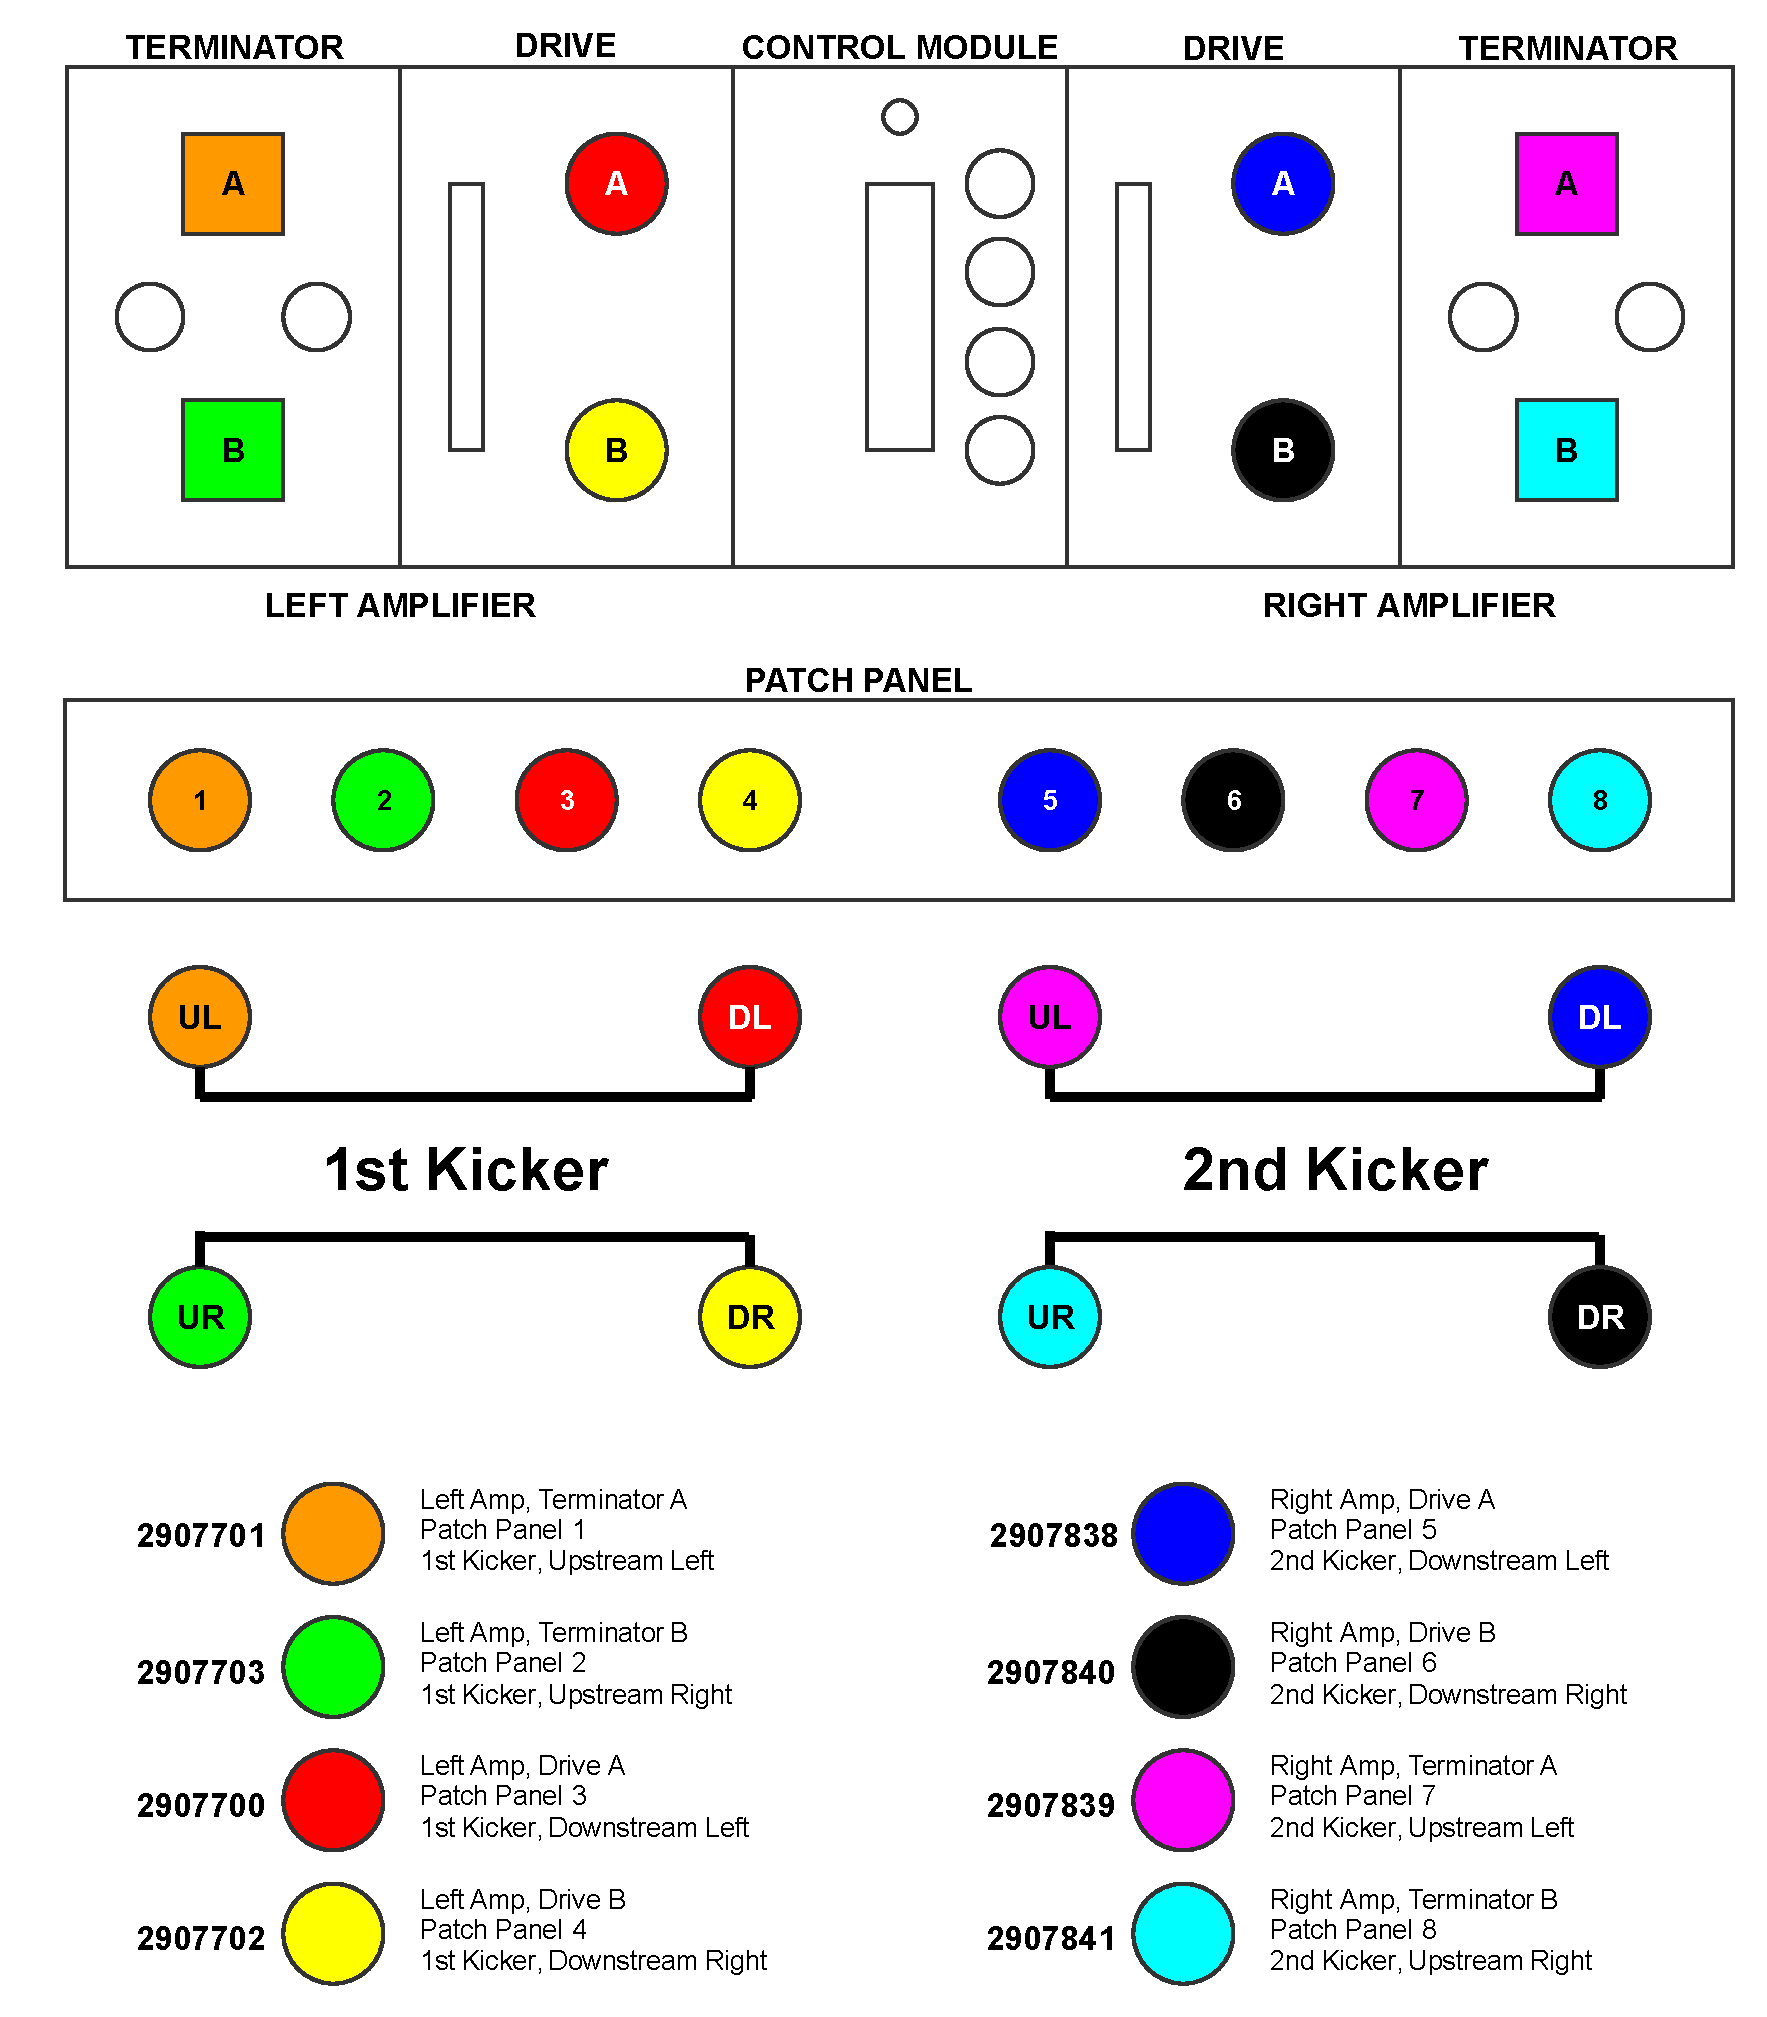
\includegraphics[width=0.9\textwidth]{Figures/commissioning/kickerCables}
  \caption{Cabling setup for cables between the amplifier and kickers.}
  \label{f:kickerCables}
\end{figure}




\subsection{Linearity}
\label{ss:ampLin}

Figure \ref{f:AmpOutvsDAC} shows the amplifier output, as measured by the monitoring signals, at different constant input voltages sent from the FONT5a board between the minimum of -2V (-4096 DAC counts) and maximum of 2V (+4096 DAC counts) [TODO: One of these 4095 not 4096?]. The output voltage from the monitoring signals is converted in to the real amplifier output Voltage using the approximate conversion factor of 115. All four amplifier outputs are shown (one for each strip of the two kickers). The plotted values are means taken across a 480~ns central part of the whole 1400~ns [TODO: Check - looks more like 1500 ns in data] output pulse.

The relative polarity of the four outputs is equivalent to what would be sent to the kickers during PFF operation, with opposite polarity of the L and R amplifier outputs sent to each kicker, so that the beam is kicked in opposite directions by each kicker with the second kicker then closing the orbit bump created by the first. Within each side of the amplifier the A and B outputs (sent to each side of the kicker) also have opposite polarity, necessary to create the potential difference across the strips within each kicker that creates the deflecting field for the beam. The relative polarity of the A and B outputs is fixed in the amplifier design and can not be controlled via the FONT5a board.

The response of the amplifier is highly linear in the region between \(\pm1.2\)~V sent to the amplifier. Outside this range the amplifier clearly begins to enter saturation, in particular above input voltages of \(\pm1.7\)~V. The linear fits shown include only the points between \(\pm1.2\)~V, excluding the first and last three points in the scan of input voltages, in order to not be biased by the effects of saturation.

Figure \ref{f:AmpOutvsDAC_residual} shows the residuals between the linear fit and the real amplifier output across the full range of input voltages. By looking at the residuals a slight deviation from linearity in the \(\pm1.2\)~V range is also visible, although the maximum difference is only 10~V or a 3\% relative error. At the maximum input voltage of \(\pm2\)~V the difference between the real output and the amplitude expected if the response was linear across the full range rises above 150~V, or a relative error of more than 25\%. For example, the RB output at an input voltage of \(+2\)~V is 605~V but the fitted response gives 769~V, a difference of 164~V or 27\%.

The effects of amplifier saturation are not taken in to account in the PFF algorithm on the FONT5a board, in which the DAC output is linearly dependent on the input phase (voltage from the phase monitor mixer signal) across the full range. The applied correction to the downstream phase will therefore be non-optimal when the DAC output calculated by the PFF algorithm is above an absolute value of 2500 counts (1.2~V sent to the amplifier). [TODO: Calculate how significant later?]

Differences in the gradient and peak output - real or just monitoring calibration?
If real effect on PFF - difference between kickers means non-closed orbit. Difference between strips just changes phase vs. input voltage, no issue as long as linear.

\begin{figure}
  \centering
  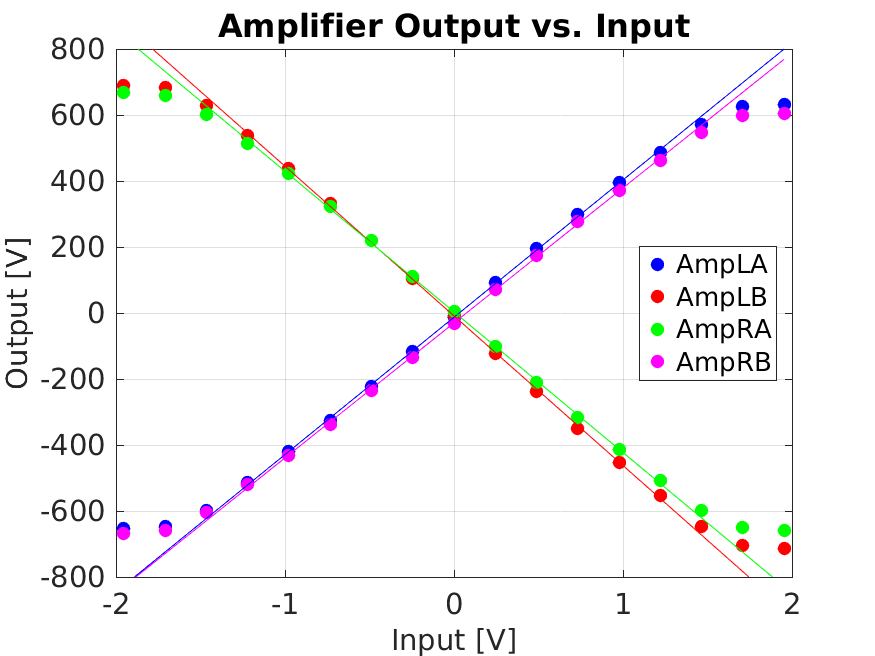
\includegraphics[width=0.9\textwidth]{Figures/commissioning/AmpOutvsDAC}
  \caption{Amplifier output vs. input.}
  \label{f:AmpOutvsDAC}
\end{figure}

\begin{figure}
  \centering
  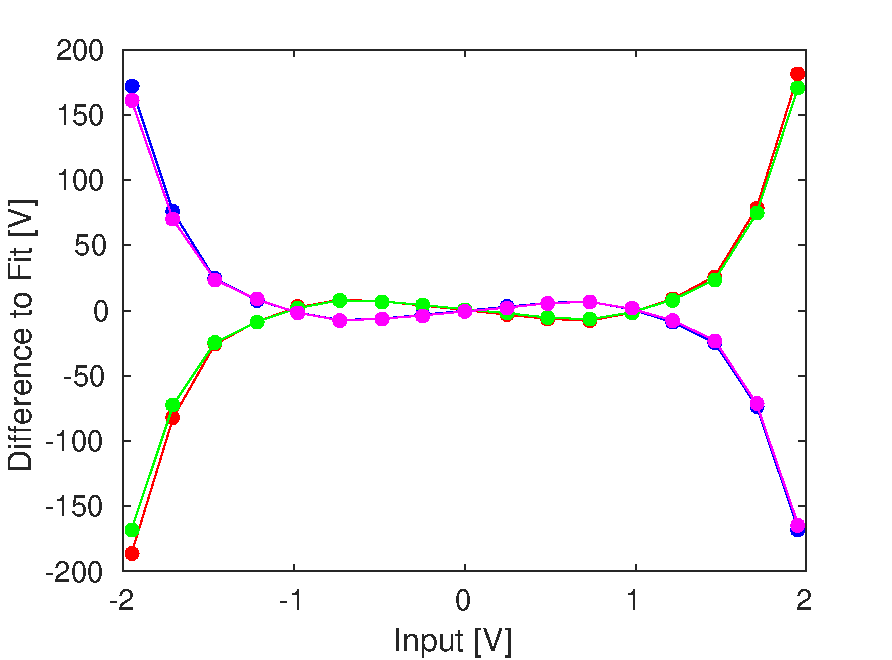
\includegraphics[width=0.9\textwidth]{Figures/commissioning/AmpOutvsDAC_residual}
  \caption{Residual between amplifier output and linear fit.}
  \label{f:AmpOutvsDAC_residual}
\end{figure}

\begin{table}
  \begin{center}
    \begin{tabular}{| c | c |}
	   \hline
       Amplifier Port & Output at +1~V Input \\ \hline
       LA & \(+416\pm3\)~V \\
	   LB & \(-453\pm3\)~V \\
	   RA & \(-426\pm3\)~V \\
	   RB & \(+409\pm3\)~V \\
 	   \hline
    \end{tabular}
    \caption{Feedforward results using combined data from 20th November 2015.}
  	\label{t:AmpOutVsDAC}
  \end{center}
\end{table}

http://accelconf.web.cern.ch/accelconf/ipac2011/papers/tupc007.pdf
1.4 kV to each strip = 1 mrad kick at 150 MeV
1.26 kV to each strip = 1 mrad kick at 135 MeV

\subsection{Shape}
\label{ss:ampShape}


\subsection{Bandwidth}
\label{ss:ampBand}

\newsection{daqSigProc}{Data Acquisition and Signal Processing}

\subsection{SiS Digitiser Setup}
\label{ss:sisSetup}

(already discussed in ph mon chapter)

\subsection{Acquisition Tools}
\label{ss:acqTools}

\subsection{Monitoring Tools}
\label{ss:monTools}

Online display

\subsection{Time Alignment of Signals}
\label{ss:timeAlignment}

\subsection{Definition of Zero Phase}
\label{ss:zeroPhase}

\newsection{constKicks}{Kicker and Optics Performance Verification}

\subsection{Correction Range}
\label{ss:corrRange}

Scan and comparison to expectation from optics.

Effect on correction.

Optics: 0.7m R52 -> 10 degrees for 1mrad kick


\subsection{Linearity}
\label{ss:kickLin}

\subsection{Orbit Closure}
\label{ss:orbitClosure}

\subsection{Shape}
\label{ss:kickShape}

Shape of FF kick on BPMs vs. shape of upstream phase

\newsection{timing}{Correction Output Timing}

\subsection{Latency}
\label{ss:measLatency}

\subsection{Absolute Timing}
\label{ss:absTiming}

\subsubsection{Using Beam Pickup}
\label{sss:beamPickup}

\subsubsection{Using BPMs}
\label{sss:relativeBPM}

\subsection{Relative Kicker Timing}
\label{ss:relativeTiming}

\begin{figure}
  \centering
  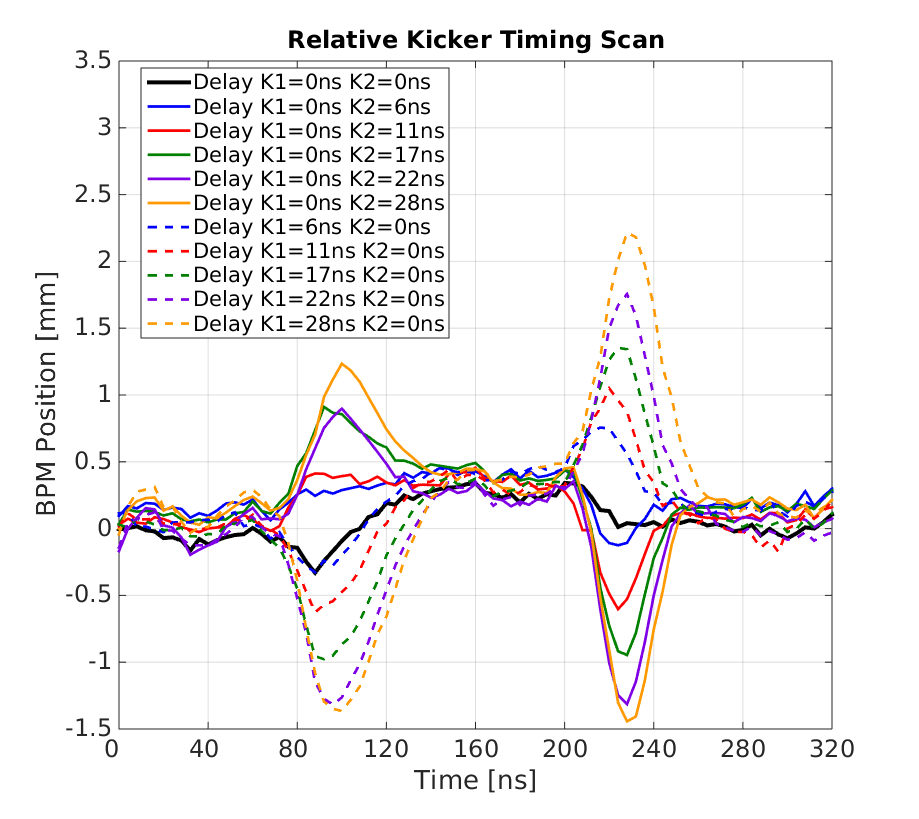
\includegraphics[width=0.45\textwidth]{Figures/commissioning/relativeTimingScan_traces}
  \caption{Traces relative timing scan.}
  \label{f:relativeTimingScan_traces}
\end{figure}

\begin{figure}
  \centering
  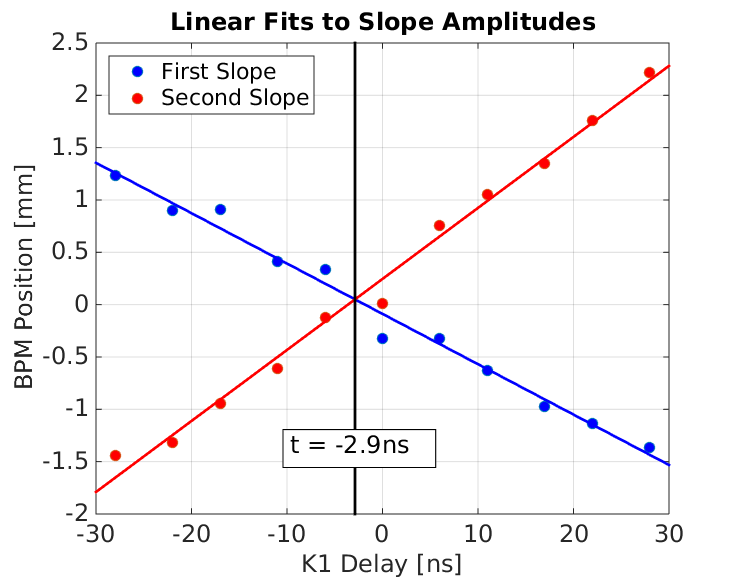
\includegraphics[width=0.45\textwidth]{Figures/commissioning/relativeTimingScan_slopeFit}
  \caption{Relative timing scan - fit to rising/falling edge.}
  \label{f:relativeTimingScan_slopeFit}
\end{figure}



%\newsection{corrBandwidth}{Correction Bandwidth}




